\scnstructheader{Описание подсистемы взаимодействия c sc-памятью на основе языка JSON}
\scnstartsubstruct

\scnheader{Реализация подсистемы взаимодействия c sc-памятью на основе языка JSON}
\scnexplanation{Реализация подсистемы взаимодействия c sc-памятью на основе языка JSON позволяет ostis-системам взаимодействовать с системами из внешней среды на основе общепринятого транспортного формата передачи данных JSON и предоставляет API для доступа к sc-памяти платформы интерпретации sc-моделей.}
\scnrelfromlist{используемый язык программирования}{C;C++;Python;TypeScript;C\#;Java}
\scnrelfromlist{используемый язык}{SC-JSON-код}
\scnrelfrom{архитектура}{Клиент-серверная архитектура}
\scnrelto{реализация}{Подсистема взаимодействия с sc-памятью на основе языка JSON}
\scnaddlevel{1}
	\scnidtf{Подсистема взаимодействия с sc-памятью на основе формата JSON}
	\scnidtf{Подсистема взаимодействия с sc-памятью на основе транспортного формата передачи данных JSON}
	\scniselement{многократно используемый компонент ostis-систем}
	\scniselement{неатомарный многократно используемый компонент ostis-систем}
	\scniselement{зависимый многократно используемый компонент ostis-систем}
	\scnrelfromlist{авторы}{Корончик Д. Н.\\; Шункевич Д. В.\\; Зотов Н. В.\\; Загорский А. Г.}
	\scnexplanation{Взаимодействие c sc-памятью обеспечивается с помощью передачи информации на \textit{\textbf{SC-JSON-коде}} и ведётся, с одной стороны, между сервером, являющегося частью ostis-системы, написанным на том же языке реализации этой ostis-системы и имеющим доступ к её sc-памяти, и с другой стороны множеством клиентом, которым известно о наличии сервера в пределах сети их использования.}
	\scnnote{Осмысленные фрагменты текстов \textit{\textbf{SC-JSON-кода}} представляют семантически корректную структуру сущностей и связей между ними.}
	\scnnote{С помощью подсистемы взаимодействия с sc-памятью на основе языка JSON можно взаимодействовать с ostis-системой на таком же множестве возможных операций, как и в случае, если бы взаимодействие происходило (непосредственно) напрямую, на том же языке реализации платформы интерпретации sc-моделей компьютерных систем. При этом результат работы отличается только скоростью обработки информации.}
	\scnrelfromset{декомпозиция программной системы}{
		Серверная система на основе Websocket, обеспечивающая доступ к sc-памяти платформы интерпретации sc-моделей при помощи команд SC-JSON-кода\\;
		Множество клиентских систем, подключаемых и взаимодействующих с \textit{Серверной системой на основе Websocket, обеспечивающей доступ к sc-памяти платформы интерпретации sc-моделей при помощи команд SC-JSON-кода}\\
		\scnaddlevel{1}
			\scnrelfromset{декомпозиция программной системы}{
				Клиентская система, подключаемая и взаимодействующая с \textit{SC-сервером}, реализованная на языке программирования Python\\;
				Клиентская система, подключаемая и взаимодействующая с \textit{SC-сервером}, реализованная на языке программирования TypeScript\\;
				Клиентская система, подключаемая и взаимодействующая с \textit{SC-сервером}, реализованная на языке программирования C\#\\;
				Клиентская система, подключаемая и взаимодействующая с \textit{SC-сервером}, реализованная на языке программирования Java
		}
		\scnaddlevel{-1}
}
\scnaddlevel{-1}

\scnheader{SC-JSON-код}
\scnidtf{Semantic JSON-code}
\scnidtf{Semantic JavaScript Object Notation code}
\scnidtf{Язык внешнего смыслового представления знаний для взаимодействия с ostis-системами на основе языка JSON}
\scnidtf{Метаязык, являющийся подмножеством языка JSON и обеспечивающий внешнее представление и структуризацию \textit{sc-текстов}, используемых ostis-системой в процессе своего функционирования и взаимодействия со внешней средой.}
\scntext{часто используемый неосновной внешний идентификатор sc-элемента}{sc-json-текст}
\scnaddlevel{1}
	\scniselement{имя нарицательное}
\scnaddlevel{-1}
\scniselement{абстрактный язык}
\scniselement{линейный язык}
\scnsubset{JSON}
\scnrelfromlist{авторы}{Зотов Н. В.\\; Корончик Д. Н.}
\filemodetrue
\scnrelfromvector{принципы, лежащие в основе}{Тексты, описываемые на языке внешнего представления знаний \textit{\textbf{SC-JSON-код}} представляют собой линейную структуру, представляемую в виде линейного строкового текста и состоящую из набора корректных осмысленных команд, записанных в виде \textit{sc-json-пар} вида \{отношение: объект\}, где отношением выступает знак квазибинарного отношения, состоящего из пар вида \{субъект: объект\}, где объектом выступает знак, обозначаемый предложением, включающее такие пары, а субъектом - sc-json-объекты: sc-json-литерал, sc-json-списки sc-json-объектов, sc-json-предложения, состоящие из sc-json-списков sc-json-объектов; 
Тексты \textit{\textbf{SC-JSON-кода}} представляют собой sc-json-команды. Каждая команда представляет собой json-объект, в котором указываются уникальный идентификатор команды, тип этой команды и ее аргументы. C каждой командой ассоциируется ответ на эту команду. Ответ на команду представляет собой команду, в котором указываются идентификатор команды, ее статус (выполнена успешно/безуспешно) и результаты. Структура аргументов и результатов команды определяется типом команды. Для каждого ответа существует запрос.}
\filemodefalse 
\scnrelfromlist{достоинство}{\scnfileitem{Язык JSON является общепринятым открытым форматом, для работы с которым существует большое количество библиотек для популярных языков программирования. Это, в свою очередь, упрощает реализацию клиента и сервера для протокола, построенного на базе \textit{\textbf{SC-JSON-код}}.};
\scnfileitem{Реализация подсистемы взаимодействия со внешней средой на базе \textit{\textbf{SC-JSON-код}} не накладывает принципиальных ограничений на объем (длину) каждой команды, в отличие от других бинарных протоколов. Таким образом, появляется возможность использования неатомарных команд, позволяющих, например, за один акт пересылки такой команды по сети создать сразу несколько sc-элементов. Важными примерами таких команд являются \textit{команда создания sc-конструкции, изоморфной заданному sc-шаблону}, и \textit{команда поиска sc-конструкций, изоморфных заданному sc-шаблону}.}}
\scnnote{Можно сказать, что язык на базе JSON является следующим шагом на пути к созданию мощного и универсального языка запросов, аналогичного языку SQL для реляционных баз данных и предназначенному для работы с sc-памятью. Следующий шагом станет реализация такого протокола на основе одного из стандартов внешнего отображения sc-конструкций, например, \textit{SCs-кода}, что, в свою очередь, позволит передавать в качестве команд целые программы обработки sc-конструкций, например на языке SCP.}

\scnstructheader{Синтаксис SC-JSON-кода}
\scnstartsubstruct
\scnheader{Синтаксис SC-JSON-кода}
\scnnote{\textit{Синтаксис SC-JSON-кода} задается: (1) \textit{Алфавитом SC-JSON-кода}, (2) Грамматикой SC-JSON-кода}
\scnrelto{синтаксис}{SC-JSON-код}

\scnstructheader{Синтаксическая классификация элементов SC-JSON-кода}
\scnstartsubstruct

\scnstructheader{SC-JSON-код}
\scnrelto{семейство подмножеств}{sc-json-предложение}
\scnaddlevel{1}
	\scnsubset{json-список json-пар}
	\scnrelto{семейство подмножеств}{sc-json-пара*}
	\scnaddlevel{1}
		\scnreltovector{декартово произведение}{
			sc-json-строка\\;
			sc-json-объект\\
			\scnaddlevel{1}
				\scnsubdividing
				{
					sc-json-cписок\\;
					sc-json-пара\\;
					sc-json-литерал\\
					\scnaddlevel{1}
						\scnsubdividing
						{
							sc-json-строка\\;
							sc-json-число
						}
					\scnaddlevel{-1}
				}
			}
		\scnaddlevel{-1}
	\scnaddlevel{-1}
	\scnsubdividing
	{
		команда на SC-JSON-коде\\;
		ответ на команду на SC-JSON-коде
	}
\scnaddlevel{-1}

\scnendstruct \scninlinesourcecommentpar{Завершили представление \textit{Синтаксической классификации элементов SC-JSON-кода}}

\scnheader{Алфавит SC-JSON-кода\scnsupergroupsign}
\scnidtf{Множество всех возможных символов в SC-JSON-коде}
\scnexplanation{Поскольку SC-JSON-код является линейным строковым языком представления знаний, то его алфавит включает объединение алфавитов всех языков, тексты на которых могут представлять внешние идентификаторы и/или содержимое файлов ostis-системы, множество всех цифр и множество всех других специальных символов.}
\scnrelto{алфавит}{SC-JSON-код}
\scnnote{Последовательности знаков алфавита могут образовывать sc-json ключевые слова, sc-json-пары, sc-json-предложения из sc-json-пар и sc-json-тексты из sc-json-предложений.}

\scnheader{SC-JSON-код}
\scnrelfromlist{синтаксические правила}{\scnfileitem{Каждое правило \textit{Грамматики SC-JSON-кода} описывает корректный с точки зрения \textit{Синтаксиса SC-JSON-кода} порядок sc-json-объектов в sc-json-предложении. Совокупность правил \textit{Грамматики SC-JSON-кода} описывает корректный с точки зрения \textit{Синтаксиса SC-JSON-кода} порядок sc-json-предложений в sc-json-тексте.};
\scnfileitem{Каждое sc-json-предложение является sc-json-списком, состоящим из sc-json-пар и представляет собой команду или ответ на эту команду.};
\scnfileitem{Каждое \textit{команда (ответ на команду) на SC-JSON-коде} состоит из заголовка, включающего sc-json-пары описания самой команды (ответа на команду), и сообщения, различного для каждого класса команд (ответов на команды). Сообщение {команды (ответа на команду) на SC-JSON-коде} обычно представляет собой список sc-json-объектов и может не ограничиваться по мощности.};
\scnfileitem{Каждая sc-json-пара состоит из двух элементов: ключевого слова и некоторого другого sc-json-объекта, ассоциируемого с этим ключевым словом. Набор ключевых слов в sc-json-парах определяется конкретным классом {команд (ответов на команды) на SC-JSON-коде}. Sc-json-пара начинается знаком открывающейся фигурной скобки "\{"{} и заканчивается знаком закрывающейся фигурной скобки "\}". Ключевое слово и sc-json-объект, ассоциируемый с ним, разделяются при помощи знака двоеточия ":".};
\scnfileitem{Sc-json-строки, записанные в sc-json-текстах, начинаются и заканчиваются знаком двух ковычек \textquotedblleft.};	\scnfileitem{Sc-json-списки, состоящие не из sc-json-пар, начинаются знаком открывающейся квадратной скобки "["{} и заканчиваются знаком закрывающейся квадратной скобки "]". Sc-json-объекты в sc-json-списках разделяются запятыми ",".}}

\scnheader{Грамматика SC-JSON-кода}
\scnidtf{Множество всех возможных правил, используемых при построении команд и ответов на них на SC-JSON-коде}
\scnexplanation{Каждой команде \textit{SC-JSON-кода} однозначно соответствует правило грамматики \textit{SC-JSON-кода}.}
\scnrelto{грамматика}{SC-JSON-код}
\scnexplanation{Правила \textit{Грамматики SC-JSON-кода} позволяют правильно составить команду на SC-JSON-коде. Каждое правило грамматики \textit{SC-JSON-кода} представляется в виде правила на \textit{Языке описания грамматик ANTLR} и его интерпретации на естественном языке.}

\scnhaselementrole{ключевой sc-элемент}{Правило, задающее синтаксис \textit{команд на SC-JSON-коде}}
\scnaddlevel{1}
	\scnrelboth{семантическая эквивалентность}{\scnfileimage{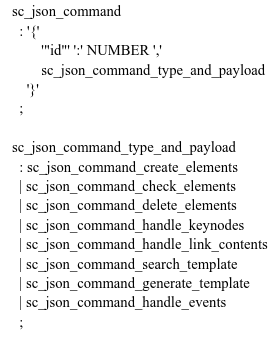
\includegraphics[scale=0.95]{images/command}}}
	\scnaddlevel{1}
		\scniselement{Язык описания грамматики языков ANTLR}
		\scntext{интерпретация}{Класс \textit{команд на SC-JSON-коде} включает \textit{команду создания sc-элементов}, \textit{команду получения соответствующих типов sc-элементов}, \textit{команду удаления sc-элементов}, \textit{команду обработки ключевых sc-элементов}, \textit{команду обработки содержимого файлов ostis-системы}, \textit{команду поиска sc-конструкций, изоморфных заданному sc-шаблону}, \textit{команду генерации sc-конструкции, изоморфной заданному sc-шаблону}, и \textit{команду обработки sc-событий}. В \textit{команду на SC-JSON-коде} включаются идентификатор этой команды, тип и сообщение.}
	\scnaddlevel{-1}
	\scnrelto{синтаксическое правило}{команда на SC-JSON-коде}
\scnaddlevel{-1}

\scnhaselementrole{ключевой sc-элемент}{Правило, задающее синтаксис \textit{ответа на команду на SC-JSON-коде}}
\scnaddlevel{1}
	\scnrelboth{семантическая эквивалентность}{\scnfileimage{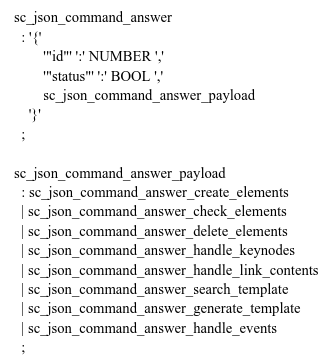
\includegraphics[scale=0.95]{images/command_answer}}}
	\scnaddlevel{1}
		\scniselement{Язык описания грамматики языков ANTLR}
		\scntext{интерпретация}{Класс \textit{ответов на команды на SC-JSON-коде} включает \textit{ответ на команду создания sc-элементов}, \textit{ответ на команду получения соответствующих типов sc-элементов}, \textit{ответ на команду удаления sc-элементов}, \textit{ответ на команду обработки ключевых sc-элементов}, \textit{ответ на команду обработки содержимого файлов ostis-системы}, \textit{ответ на команду поиска sc-конструкций, изоморфных заданному sc-шаблону}, \textit{ответ на команду генерации sc-конструкции, изоморфной заданному sc-шаблону}, и \textit{ответ на команду обработки sc-событий}. В \textit{ответ на команду на SC-JSON-коде} включаются идентификатор соответствующей команды, статус обработки ответа и ответное сообщение.}
	\scnaddlevel{-1}
	\scnrelto{синтаксическое правило}{ответ на команду на SC-JSON-коде}
\scnaddlevel{-1}

\scnhaselement{Правило, задающее синтаксис \textit{команды создания sc-элементов}}
\scnaddlevel{1}
	\scnrelboth{семантическая эквивалентность}{\scnfileimage{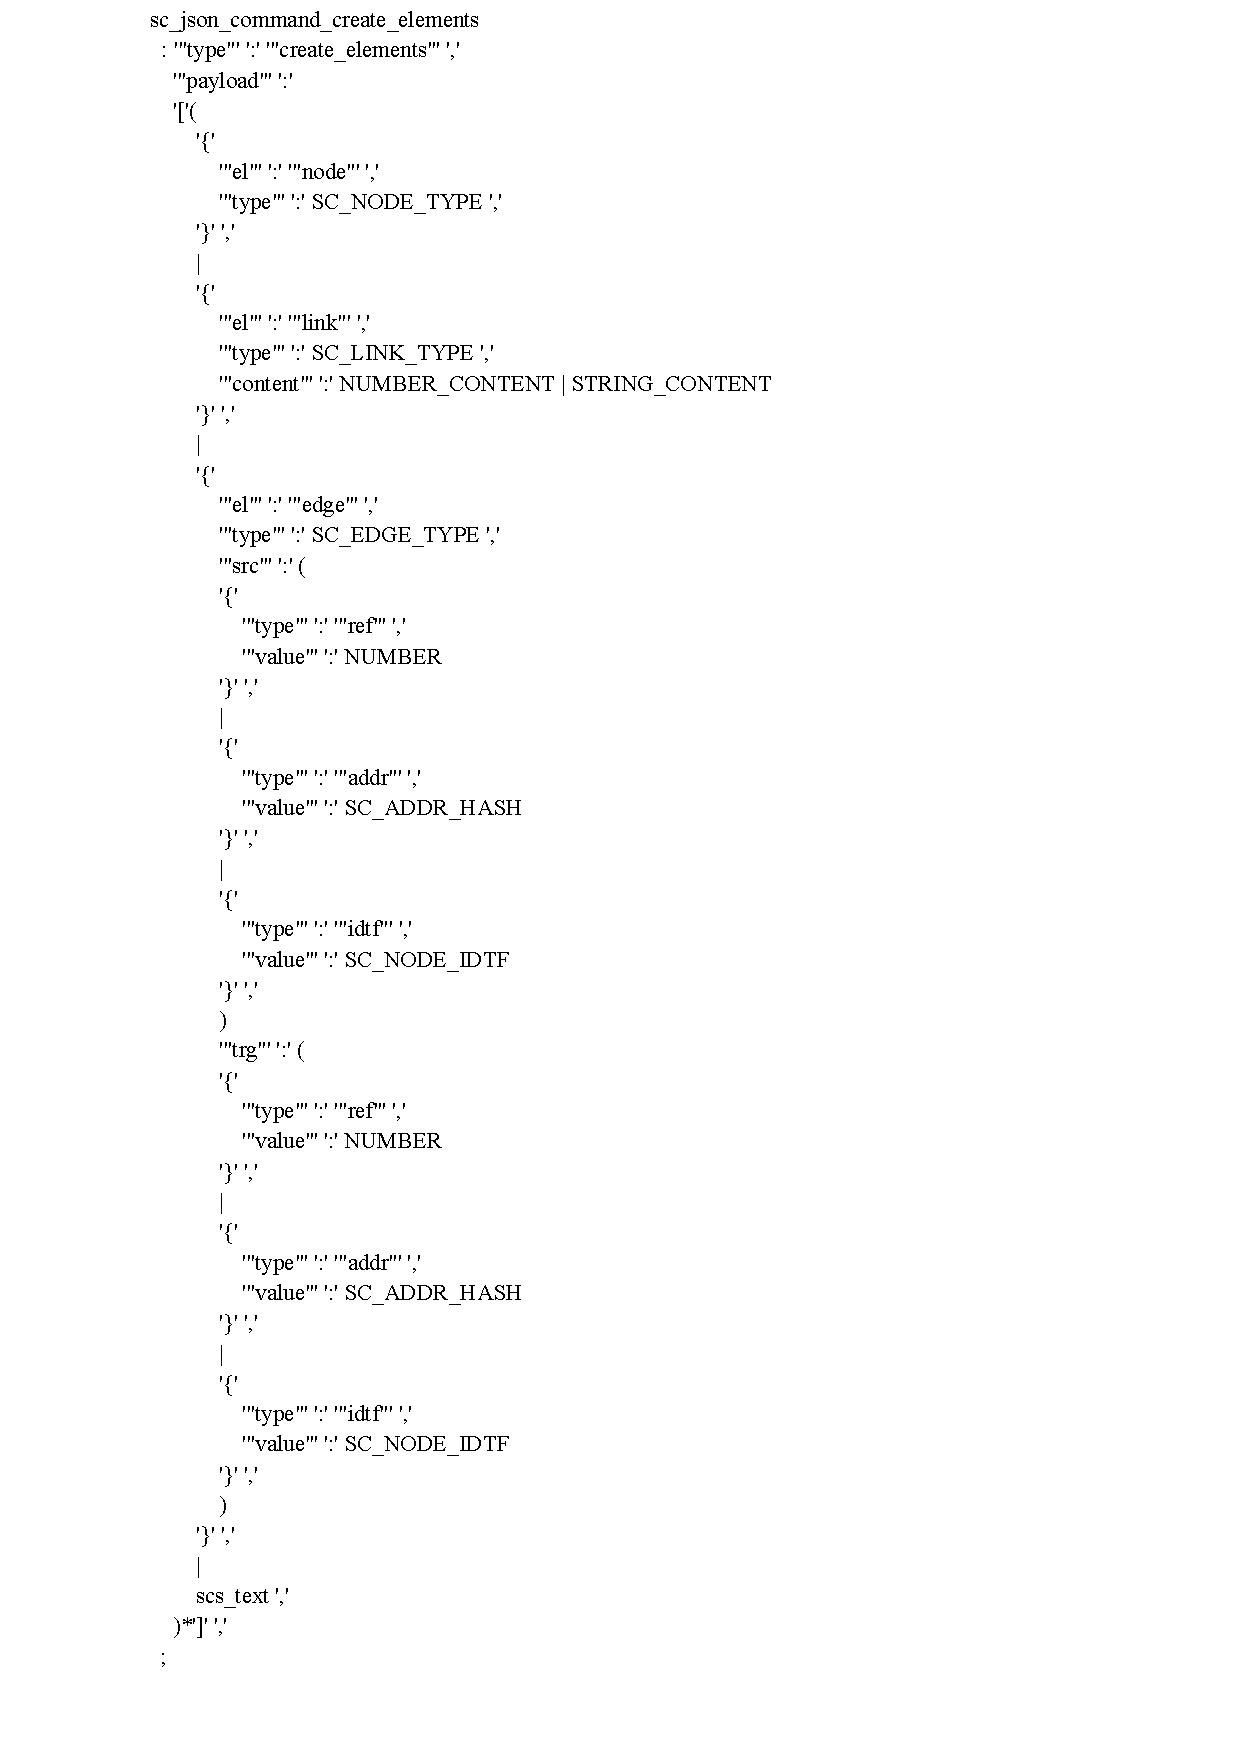
\includegraphics[scale=0.95]{images/create_elements_command}}}
	\scnaddlevel{1}
		\scniselement{Язык описания грамматики языков ANTLR}
		\scntext{интерпретация}{В сообщении \textit{команды создания sc-элементов} представляется список описаний создаваемых sc-элементов. Такими sc-элементами могут быть sc-узел, sc-дуга, sc-ребро или файл ostis-системы. Тип sc-элемента указывается в паре с ключевым словом "el"{}: для sc-узла sc-json-тип элемент представляется как "node"{}, для sc-дуги и sc-ребра - "edge"{}, для файла ostis-системы - "link". Метки типов sc-элементов уточняются в соответствующих им описаниях в сообщении команды в паре с ключевым словом "type". Если создаваемым sc-элементом является файл ostis-системы, то дополнительно указывается содержимое этого файла ostis-системы в паре с ключевым словом "content"{}, если создаваемым sc-элементом является sc-дуга или sc-ребро, то указываются описания sc-элементов, из которых они выходят, и sc-элементов, в которые они входят. Описание таких sc-элементов состоят из двух пар: первая пара указывает на способ ассоциации с sc-элементом и представляется как "addr"{} или "idtf"{} или "ref"{} в паре с ключевым словом "type"{}, вторая пара - то, по чему происходит ассоциация с этим sc-элементом: его хэшу, системному идентификатору или номеру в массиве создаваемых sc-элементов - в паре с ключевым словом "value".}
	\scnaddlevel{-1}
	\scnrelto{синтаксическое правило}{команда создания sc-элементов}
\scnaddlevel{-1}

\scnhaselement{Правило, задающее синтаксис \textit{ответа на команду создания sc-элементов}}
\scnaddlevel{1}
	\scnrelboth{семантическая эквивалентность}{\scnfileimage{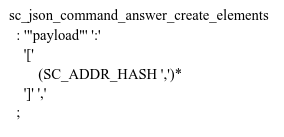
\includegraphics[scale=0.95]{images/create_elements_command_answer}}}
	\scnaddlevel{1}
		\scniselement{Язык описания грамматики языков ANTLR}
		\scntext{интерпретация}{Сообщением \textit{ответа на команду создания sc-элементов} является список хэшей созданных sc-элементов, соответствующих описаниям \textit{команды создания sc-элементов} со статусом 1, в случае успешной обработки команды.}
	\scnaddlevel{-1}
	\scnrelto{синтаксическое правило}{ответ на команду создания sc-элементов}
\scnaddlevel{-1}

\scnhaselement{Правило, задающее синтаксис \textit{команды получения соответствующих типов sc-элементов}}
\scnaddlevel{1}
	\scnrelboth{семантическая эквивалентность}{\scnfileimage{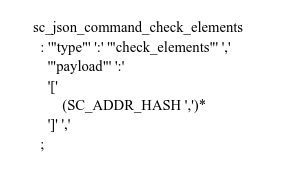
\includegraphics[scale=0.95]{images/check_elements_command}}}
	\scnaddlevel{1}
		\scniselement{Язык описания грамматики языков ANTLR}
		\scntext{интерпретация}{Сообщением \textit{команды получения соответствующих типов sc-элементов} является списком хэшей sc-элементов, у которых необходимо получить синтаксические типы.}
	\scnaddlevel{-1}
	\scnrelto{синтаксическое правило}{команда получения соответствующих типов sc-элементов}
\scnaddlevel{-1}

\scnhaselement{Правило, задающее синтаксис \textit{ответа на команду получения соответствующих типов sc-элементов}}
\scnaddlevel{1}
	\scnrelboth{семантическая эквивалентность}{\scnfileimage{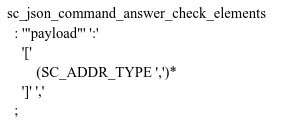
\includegraphics[scale=0.95]{images/check_elements_command_answer}}}
	\scnaddlevel{1}
		\scniselement{Язык описания грамматики языков ANTLR}
		\scntext{интерпретация}{Сообщением \textit{ответа на команду получения соответствующих типов sc-элементов} является список типов проверенных sc-элементов, соответствующих описаниям \textit{команды получения соответствующих типов sc-элементов} со статусом 1, в случае успешной обработки команды.}
	\scnaddlevel{-1}
	\scnrelto{синтаксическое правило}{ответ на команду получения соответствующих типов sc-элементов}
\scnaddlevel{-1}

\scnhaselement{Правило, задающее синтаксис \textit{команды удаления sc-элементов}}
\scnaddlevel{1}
	\scnrelboth{семантическая эквивалентность}{\scnfileimage{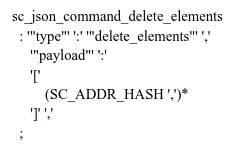
\includegraphics[scale=0.95]{images/delete_elements_command}}}
	\scnaddlevel{1}
		\scniselement{Язык описания грамматики языков ANTLR}
		\scntext{интерпретация}{Сообщением \textit{команды удаления sc-элементов} является список хэшей sc-элементов, которые необходимо удалить из sc-памяти.}
	\scnaddlevel{-1}
	\scnrelto{синтаксическое правило}{команда удаления sc-элементов}
\scnaddlevel{-1}

\scnhaselement{Правило, задающее синтаксис \textit{ответа на команду удаления sc-элементов}}
\scnaddlevel{1}
	\scnrelboth{семантическая эквивалентность}{\scnfileimage{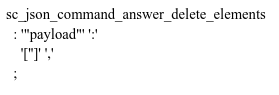
\includegraphics[scale=0.95]{images/delete_elements_command_answer}}}
	\scnaddlevel{1}
		\scniselement{Язык описания грамматики языков ANTLR}
		\scntext{интерпретация}{Сообщение \textit{ответа на команду удаления sc-элементов} является пустым со статусом 1, в случае успешной обработки команды.}
	\scnaddlevel{-1}
	\scnrelto{синтаксическое правило}{ответ на команду удаления sc-элементов}
\scnaddlevel{-1}

\scnhaselement{Правило, задающее синтаксис \textit{команды обработки ключевых sc-элементов}}
\scnaddlevel{1}
	\scnrelboth{семантическая эквивалентность}{\scnfileimage{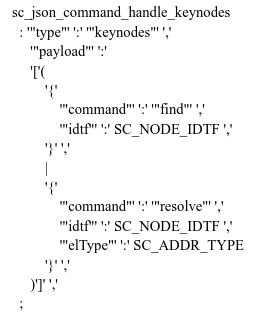
\includegraphics[scale=0.95]{images/handle_keynodes_command}}}
	\scnaddlevel{1}
	\scniselement{Язык описания грамматики языков ANTLR}
	\scntext{интерпретация}{Сообщение \textit{команды обработки ключевых sc-элементов} может включать описание ключевых sc-элементов, которые необходимо найти и/или разрешить по их идентификаторам. Такое деление осуществляется с помощью подкоманд, содержащихся в сообщении команды. Идентификаторами подкоманд могут быть "find"{} и "resolve"{} соответственно, стоящие в паре с ключевым словом "command". Описание искомого sc-элемента команды "find"{} включает системный идентификатор sc-элемента, по которому необходимо найти этот sc-элемент, стоящий в паре с ключевым словом "idtf". Описание разрешаемого sc-элемента команды "resolve"{} включает системный идентификатор sc-элемента, по которому необходимо найти этот sc-элемент, либо в случае безуспешного поиска создать sc-элемент некоторого типа, указанного в его описании в паре с ключевым словом "elType"{}, и установить для него системный идентификатор, по которому была произведена попытка найти другой sc-элемент.}
	\scnaddlevel{-1}
	\scnrelto{синтаксическое правило}{команда обработки ключевых sc-элементов}
\scnaddlevel{-1}

\scnhaselement{Правило, задающее синтаксис \textit{ответа на команду обработки ключевых sc-элементов}}
\scnaddlevel{1}
	\scnrelboth{семантическая эквивалентность}{\scnfileimage{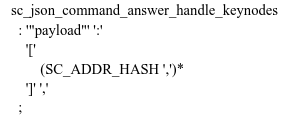
\includegraphics[scale=0.95]{images/handle_keynodes_command_answer}}}
	\scnaddlevel{1}
	\scniselement{Язык описания грамматики языков ANTLR}
	\scntext{интерпретация}{Сообщением \textit{ответа на команду обработки ключевых sc-элементов} является список хэшей sc-элементов, соответствующих описаниям \textit{команды обработки ключевых sc-элементов} со статусом 1, в случае успешной обработки команды.}
	\scnaddlevel{-1}
	\scnrelto{синтаксическое правило}{ответ на команду обработки ключевых sc-элементов}
\scnaddlevel{-1}

\scnhaselement{Правило, задающее синтаксис \textit{команды обработки содержимого файлов ostis-системы}}
\scnaddlevel{1}
	\scnrelboth{семантическая эквивалентность}{\scnfileimage{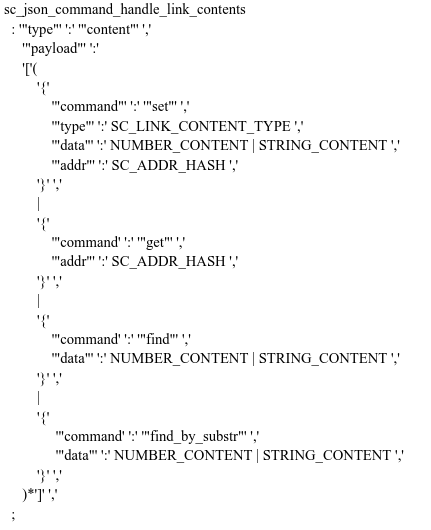
\includegraphics[scale=0.95]{images/handle_link_contents_command}}}
	\scnaddlevel{1}
		\scniselement{Язык описания грамматики языков ANTLR}
		\scntext{интерпретация}{Сообщение \textit{команды обработки содержимого файлов ostis-системы} может включать описание ключевых файлов ostis-системы, которые необходимо найти по их содержимому или части этого содержимого, для которых необходимо установить содержимое разрешить и/или у которых необходимо получить содержимое. Как и в \textit{Правиле, задающее синтаксис команды обработки ключевых sc-элементов} деление осуществляется с помощью подкоманд, содержащихся в сообщении команды. Идентификаторами подкоманд могут быть "find"{}, "find_by_substr"{}, "set"{} и "get"{} соответственно, стоящие в паре с ключевым словом "command". В описаниях команд "set"{} и "get"{} указывается хэш файла ostis-системы в паре с ключевым словом "addr". В описаниях команд "set"{}, "find"{} и "find_by_substr"{} указывается содержимое файла ostis-системы в паре с ключевым словом "data". Дополнительно в описании подкоманды "set"{} указывается тип устанавливаемого содержимого файла ostis-системы.}
	\scnaddlevel{-1}
	\scnrelto{синтаксическое правило}{команда обработки содержимого файлов ostis-системы}
\scnaddlevel{-1}

\scnhaselement{Правило, задающее синтаксис \textit{ответа на команду обработки содержимого файлов ostis-системы}}
\scnaddlevel{1}
	\scnrelboth{семантическая эквивалентность}{\scnfileimage{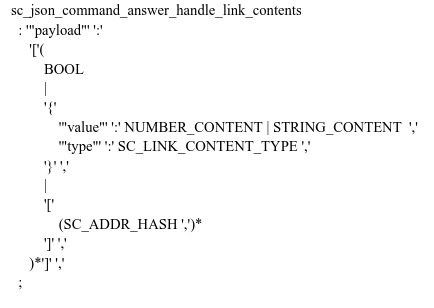
\includegraphics[scale=0.95]{images/handle_link_contents_command_answer}}}
	\scnaddlevel{1}
		\scniselement{Язык описания грамматики языков ANTLR}
		\scntext{интерпретация}{Сообщением \textit{ответа на команду обработки содержимого файлов ostis-системы} является список, состоящий из булевого результата установки содержимого в файл ostis-системы и/или найденных файлов ostis-системы по их содержимому и/или описания полученного содержимого файлов ostis-системы, соответствующих описаниям \textit{команды обработки содержимого файлов ostis-системы} со статусом 1, в случае успешной обработки команды.}
	\scnaddlevel{-1}
	\scnrelto{синтаксическое правило}{ответ на команду обработки содержимого файлов ostis-системы}
\scnaddlevel{-1}

\scnhaselement{Правило, задающее синтаксис \textit{команды поиска sc-конструкций, изоморфных заданному sc-шаблону}}
\scnaddlevel{1}
	\scnrelboth{семантическая эквивалентность}{\scnfileimage{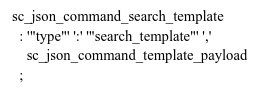
\includegraphics[scale=0.95]{images/search_template_command}}}
	\scnaddlevel{1}
		\scniselement{Язык описания грамматики языков ANTLR}
		\scnsubset{Правило, задающее синтаксис сообщения \textit{команды поиска sc-конструкций, изоморфных заданному sc-шаблону}, и \textit{команды генерации sc-конструкции, изоморфной заданному sc-шаблону}}
		\scntext{интерпретация}{\textit{Правило, задающее синтаксис команды поиска sc-конструкций, изоморфных заданному sc-шаблону} включает \textit{Правило, задающее синтаксис сообщения \textit{команды поиска sc-конструкций, изоморфных заданному sc-шаблону,} и \textit{команды генерации sc-конструкции, изоморфной заданному sc-шаблону}} и описывает команду поиска sc-конструкций по сформированному этой командой sc-шаблону (см. \textit{Правило, задающее синтаксис сообщения \textit{команды поиска sc-конструкций, изоморфных заданному sc-шаблону,} и \textit{команды генерации sc-конструкции, изоморфной заданному sc-шаблону}}).}
	\scnaddlevel{-1}
	\scnrelto{синтаксическое правило}{команда поиска sc-конструкций, изоморфных заданному sc-шаблону}
\scnaddlevel{-1}

\scnhaselement{Правило, задающее синтаксис \textit{ответа на команду поиска sc-конструкций, изоморфных заданному sc-шаблону}}
\scnaddlevel{1}
	\scnrelboth{семантическая эквивалентность}{\scnfileimage{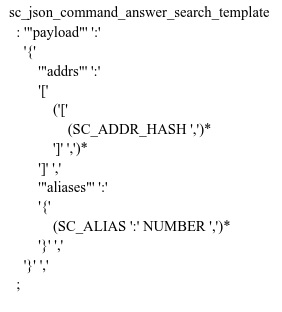
\includegraphics[scale=0.95]{images/search_template_command_answer}}}
	\scnaddlevel{1}
		\scniselement{Язык описания грамматики языков ANTLR}
		\scntext{интерпретация}{Сообщение \textit{ответа на команду поиска sc-конструкций, изоморфных заданному sc-шаблону} состоит из списка найденных sc-конструкций и отображения псевдонимов sc-элементов на их позиции в тройках sc-шаблона. Ответ имеет статус 1, в случае успешной обработки команды.}
	\scnaddlevel{-1}
	\scnrelto{синтаксическое правило}{ответ на команду поиска sc-конструкций, изоморфных заданному sc-шаблону}
\scnaddlevel{-1}

\scnhaselement{Правило, задающее синтаксис \textit{команды создания sc-конструкции, изоморфной заданному sc-шаблону}}
\scnaddlevel{1}
	\scnrelboth{семантическая эквивалентность}{\scnfileimage{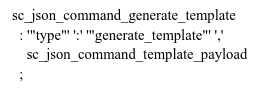
\includegraphics[scale=0.95]{images/generate_template_command}}}
	\scnaddlevel{1}
		\scniselement{Язык описания грамматики языков ANTLR}
		\scnsubset{Правило, задающее синтаксис сообщения \textit{команды поиска sc-конструкций, изоморфных заданному sc-шаблону,} и \textit{команды генерации sc-конструкции, изоморфной заданному sc-шаблону}}
		\scntext{интерпретация}{\textit{Правило, задающее синтаксис команды создания sc-конструкции, изоморфной заданному sc-шаблону} включает \textit{Правило, задающее синтаксис сообщения \textit{команды поиска sc-конструкций, изоморфных заданному sc-шаблону,} и \textit{команды генерации sc-конструкции, изоморфной заданному sc-шаблону}} и описывает команду создания sc-конструкции по сформированному этой командой sc-шаблону (см. \textit{Правило, задающее синтаксис сообщения \textit{команды поиска sc-конструкций, изоморфных заданному sc-шаблону,} и \textit{команды генерации sc-конструкции, изоморфной заданному sc-шаблону}}).}
	\scnaddlevel{-1}
	\scnrelto{синтаксическое правило}{команда создания sc-конструкции, изоморфной заданному sc-шаблону}
\scnaddlevel{-1}

\scnhaselement{Правило, задающее синтаксис \textit{ответа на команду создания sc-конструкции, изоморфной заданному sc-шаблону}}
\scnaddlevel{1}
	\scnrelboth{семантическая эквивалентность}{\scnfileimage{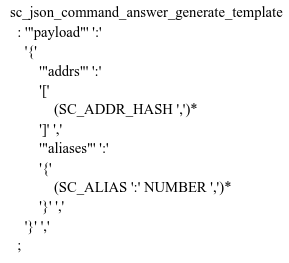
\includegraphics[scale=0.95]{images/generate_template_command_answer}}}
	\scnaddlevel{1}
		\scniselement{Язык описания грамматики языков ANTLR}
		\scntext{интерпретация}{Сообщение \textit{ответа на команду создания sc-конструкции, изоморфной заданному sc-шаблону} состоит из списка найденных sc-конструкций и отображения псевдонимов sc-элементов на их позиции в тройках sc-шаблона. Ответ имеет статус 1, в случае успешной обработки команды.}
	\scnaddlevel{-1}
	\scnrelto{синтаксическое правило}{ответ на команду создания sc-конструкции, изоморфной заданному sc-шаблону}
\scnaddlevel{-1}

\scnhaselement{Правило, задающее синтаксис сообщения \textit{команды поиска sc-конструкций, изоморфных заданному sc-шаблону,} и \textit{команды создания sc-конструкции, изоморфной заданному sc-шаблону}}
\scnaddlevel{1}
	\scnrelboth{семантическая эквивалентность}{\scnfileimage{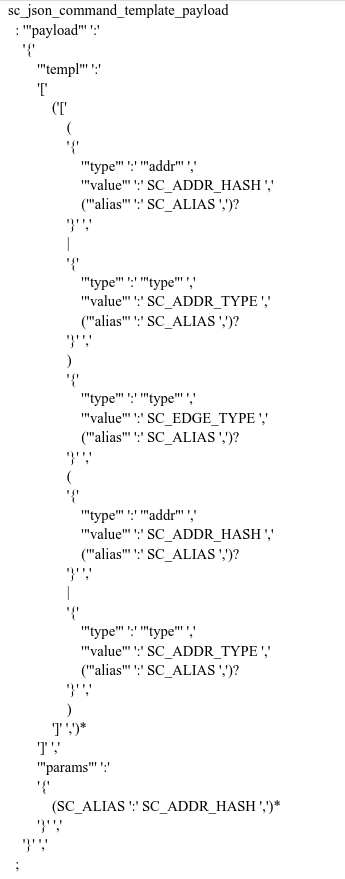
\includegraphics[scale=0.95]{images/template_message_command}}}
	\scnaddlevel{1}
		\scniselement{Язык описания грамматики языков ANTLR}
		\scntext{интерпретация}{Сообщения \textit{команды поиска sc-конструкций, изоморфных заданному sc-шаблону,} и \textit{команды создания sc-конструкции, изоморфной заданному sc-шаблону} включают описание троек, необходимых для создания sc-шаблона поиска или генерации изоморфных sc-конструкций. Описание каждой тройки sc-шаблона включает описание sc-элементов этой тройки. Описания первого и третьего sc-элементов тройки должны всегда содержать хэш или тип в паре с ключевым словом "value". Если выбран тип, то в паре с ключевым словом "type"{} указывается "type"{}, если - хэш, то - "addr"{}. Вторым sc-элементом тройки должна быть дуга, для которой всегда указывается тип в паре с ключевым словом "value". Для каждого sc-элемента тройки может указываться псевдоним в паре с "alias". Псевдоним представляет собой строку и может быть использован для ассоциации с sc-элементами в других тройках sc-шаблона, либо ассоциации со значениями переменных sc-шаблона, которые указываются в списке под ключевым словом "params"{} и могут представлять собой либо хэш sc-элемента, либо его системный идентификатор. Таким образом, в некоторых случаях может отсутствовать необходимость указания хэша или типа sc-элемента. Также вместо списка описаний троек sc-шаблона, может указываться хэш или системный идентификатор sc-структуры, хранящейся в sc-памяти. хэш и системный идентификатор указываются в паре с ключевым словом "value".}
	\scnaddlevel{-1}
\scnaddlevel{-1}

\scnhaselement{Правило, задающее синтаксис \textit{команды обработки sc-событий}}
\scnaddlevel{1}
	\scnrelboth{семантическая эквивалентность}{\scnfileimage{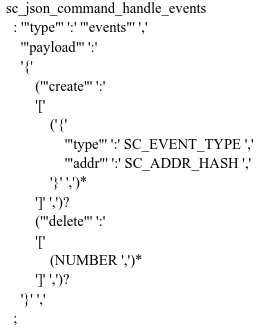
\includegraphics[scale=0.95]{images/handle_events_command}}}
	\scnaddlevel{1}
		\scniselement{Язык описания грамматики языков ANTLR}
		\scntext{интерпретация}{Сообщение \textit{команды обработки sc-событий} может включать описание sc-элементов, по котором необходимо зарегистрировать или разрегистрировать sc-события. Идентификаторами подкоманд в описании команды могут быть "create"{} и "delete"{} соответственно, стоящие в паре с ключевым словом "command". Описание команды регистрации sс-cобытий "create"{} представляет собой список описаний типов sc-событий и sc-элементов, по которым необходимо зарегистрировать sc-события. Описания sc-элементов включают хэши этих sc-элементов в парах с ключевым словом "addr". Описание команды разрегистрации sc-событий представляет собой список позиций sc-событий в очереди sc-событий, которые необходимо удалить из этой очереди sc-событий.}
	\scnaddlevel{-1}
	\scnsuperset{Правило, задающее синтаксис типов sc-событий}
	\scnaddlevel{1}
		\scnrelboth{семантическая эквивалентность}{\scnfileimage{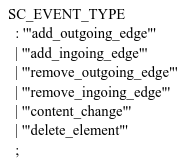
\includegraphics[scale=0.95]{images/sc_event_types}}}
		\scnaddlevel{1}
			\scniselement{Язык описания грамматики языков ANTLR}
			\scntext{интерпретация}{Sc-событиями могут быть \textit{sc-события добавления выходящей дуги из sc-элемента (add\_outgoing\_edge)}, \textit{sc-события добавления входящей дуги в sc-элемент (add\_ingoing\_edge)}, \textit{sc-события удаления выходящей дуги из sc-элемента (remove\_outgoing\_edge)}, \textit{sc-события удаления входящей дуги в sc-элемент(remove\_ingoing\_edge)}, \textit{sc-события изменения содержимого файла ostis-системы (content\_change)} и \textit{sc-события удаления sc-элемента (delete\_element)}.}
		\scnaddlevel{-1}
	\scnaddlevel{-1}
	\scnrelto{синтаксическое правило}{команда обработки sc-событий}
\scnaddlevel{-1}

\scnhaselement{Правило, задающее синтаксис \textit{ответа на команду обработки sc-событий}}
\scnaddlevel{1}
	\scnrelboth{семантическая эквивалентность}{\scnfileimage{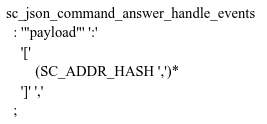
\includegraphics[scale=0.95]{images/handle_events_command_answer}}}
	\scnaddlevel{1}
		\scniselement{Язык описания грамматики языков ANTLR}
		\scntext{интерпретация}{Сообщение \textit{ответа на команду обработки sc-событий} состоит из позиций зарегистрированных sc-событий в очереди. Успешным результатом \textit{команды обработки sc-событий} является статус 1.}
	\scnaddlevel{-1}
	\scnrelto{синтаксическое правило}{ответ на команду обработки sc-событий}
\scnaddlevel{-1}

\scnhaselement{Правило, задающее синтаксис \textit{ответа инициализации sc-события}}
\scnaddlevel{1}
\scnrelboth{семантическая эквивалентность}{\scnfileimage{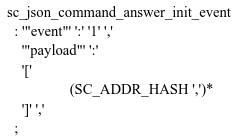
\includegraphics[scale=0.95]{images/init_event_command_answer}}}
\scnaddlevel{1}
\scniselement{Язык описания грамматики языков ANTLR}
\scntext{интерпретация}{\textit{Ответ инициализации sc-события} возникает тогда и только тогда, когда в sc-памяти инициализируется соответствующее sc-событие. \textit{Ответ инициализации sc-события} всегда отсылается той клиентской системе, которая зарегистрировала это sc-событие. В сообщение \textit{ответа инициализации sc-события} включаются хэши тех sc-элементов, которые связаны с зарегистрированным sc-событием. Таким образом, если было зарегистрировано sc-событие выходящей sc-дуги, то в списке сообщения \textit{ответа инициализации sc-события} будут находится хэши трёх sc-элементов: хэш sc-элемента, который был подписан на sc-событие, хэш добавленной выходящей из него sc-дуги и хэш sc-элемента, являющегося концом этой sc-дуги.}
\scnaddlevel{-1}
\scnrelto{синтаксическое правило}{ответ инициализации sc-события}
\scnaddlevel{-1}

\scnhaselement{Правило, задающее синтаксис \textit{синтаксических типов sc-элементов}}
\scnaddlevel{1}
\scnrelboth{семантическая эквивалентность}{\scnfileimage{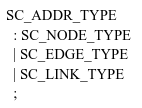
\includegraphics[scale=0.95]{images/sc_addr_types}}}
\scnaddlevel{1}
\scniselement{Язык описания грамматики языков ANTLR}
\scntext{интерпретация}{\textit{Правило, задающее синтаксис синтаксических типов sc-элементов} включает \textit{Правило, задающее синтаксис синтаксических типов sc-узлов}, \textit{Правило, задающее синтаксис синтаксических типов sc-дуг}, \textit{Правило, задающее синтаксис синтаксических типов файлов ostis-системы}. Синтаксические типы sc-элементов представляются в виде целого числа и соответствуют программным синтаксическим типам, представляемым в sc-памяти.}
\scnaddlevel{-1}
\scnnote{На данный момент форма представления синтаксического типа sc-элемента зависит от того, как располагаются биты в маске sc-элемента. Следующим шагом в развитии \textit{SC-JSON-кода} и его грамматики могли быть стать устранение такой зависимости и переход к представлению синтаксических типов в виде строковых литералов, интерпретируемых \textit{Серверной системы на основе Websocket, обеспечивающей доступ к sc-памяти платформы интерпретации sc-моделей при помощи команд SC-JSON-кода}.}
\scnaddlevel{-1}

\scnhaselement{Правило, задающее синтаксис \textit{синтаксических типов sc-узлов}}
\scnaddlevel{1}
\scnrelboth{семантическая эквивалентность}{\scnfileimage{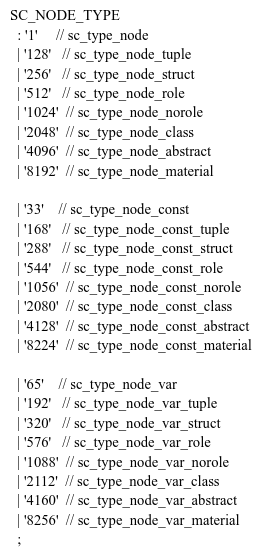
\includegraphics[scale=0.95]{images/sc_node_types}}}
\scnaddlevel{1}
\scniselement{Язык описания грамматики языков ANTLR}
\scntext{интерпретация}{\textit{Правило, задающее синтаксис синтаксических типов sc-узлов} описывает возможные синтаксические типы sc-узлов, интерпретируемые на стороне \textit{Серверной системы на основе Websocket, обеспечивающей доступ к sc-памяти платформы интерпретации sc-моделей при помощи команд SC-JSON-кода}.}
\scnaddlevel{-1}
\scnaddlevel{-1}

\scnhaselement{Правило, задающее синтаксис \textit{синтаксических типов sc-дуг}}
\scnaddlevel{1}
\scnrelboth{семантическая эквивалентность}{\scnfileimage{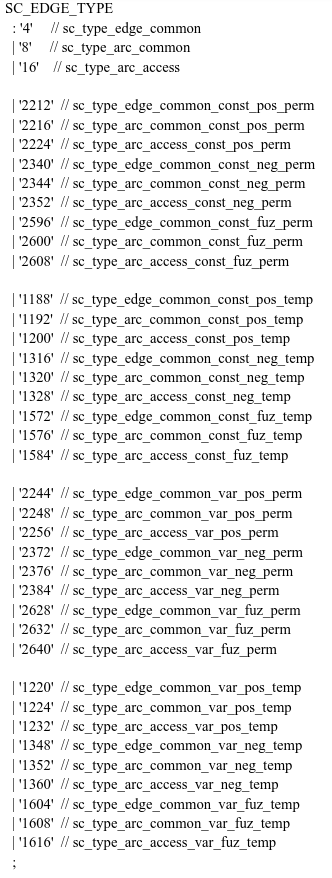
\includegraphics[scale=0.95]{images/sc_edge_types}}}
\scnaddlevel{1}
\scniselement{Язык описания грамматики языков ANTLR}
\scntext{интерпретация}{\textit{Правило, задающее синтаксис синтаксических типов sc-дуг} описывает возможные синтаксические типы sc-дуг, в том числе и sc-рёбер, интерпретируемые на стороне \textit{Серверной системы на основе Websocket, обеспечивающей доступ к sc-памяти платформы интерпретации sc-моделей при помощи команд SC-JSON-кода}.}
\scnaddlevel{-1}
\scnaddlevel{-1}

\scnhaselement{Правило, задающее синтаксис \textit{синтаксических типов файлов ostis-системы}}
\scnaddlevel{1}
\scnrelboth{семантическая эквивалентность}{\scnfileimage{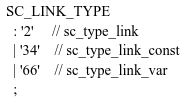
\includegraphics[scale=0.95]{images/sc_link_types}}}
\scnaddlevel{1}
\scniselement{Язык описания грамматики языков ANTLR}
\scntext{интерпретация}{\textit{Правило, задающее синтаксис синтаксических типов файлов ostis-системы} описывает возможные синтаксические типы файлов ostis-системы, интерпретируемые на стороне \textit{Серверной системы на основе Websocket, обеспечивающей доступ к sc-памяти платформы интерпретации sc-моделей при помощи команд SC-JSON-кода}.}
\scnaddlevel{-1}
\scnaddlevel{-1}

\scnheader{команда на SC-JSON-коде}
\scnidtf{sc-json-code command}
\scnsubset{SC-JSON-код}
\scnnote{Множество \textit{команд на SC-JSON-коде} легко расширяемо засчёт гибкости и функциональности языка JSON.}

\scnheader{ответ на команду на SC-JSON-коде}
\scnidtf{sc-json-code command answer}
\scnsubset{SC-JSON-код}
\scnnote{Множество \textit{ответов на команды на SC-JSON-коде} легко расширяемо вместе с расширением \textit{команд на SC-JSON-коде}.}

\scnheader{команда создания sc-элементов}
\scnidtf{create elements command}
\scnsubset{команда на SC-JSON-коде}
\scnrelfrom{пример}{Пример команды создания sc-элементов \\ \scneqfile{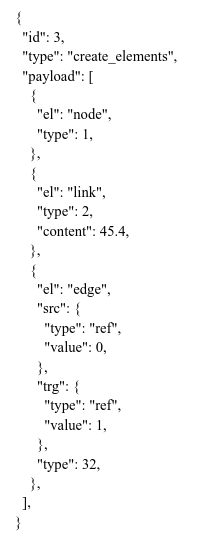
\includegraphics[scale=0.95]{images/create_elements_command_example}}}
\scnaddlevel{1}
\scniselement{команда создания sc-элементов}
\scnrelfrom{ответ}{Пример ответа на команду создания sc-элементов}
\scntext{интерпретация}{Обработать команду создания sc-элементов: sc-узла с типом 1 (неуточняемого типа), файла ostis-системы с типом 2 (неуточняемого типа) и содержимым в виде числа с плавающей точкой 45.4 и sc-дуги типа 32 (константного типа) между sc-элементом, находящимся на нулевой позиции в массиве создаваемых sc-элементов, и sc-элементом, находящимся на первой позиции в том же самом массиве.}
\scnaddlevel{-1}
\scnrelfrom{класс команд}{ответ на команду создания sc-элементов}
\scnnote{Стоит отметить, что на уровне интерфейса sc-памяти команда интерпретируется быстро за счёт того, что не используются шаблоны создания изоморфных им конструкций. Также содержимое сообщения \textit{команды создания sc-элементов} может быть пустым.}

\scnheader{ответ на команду создания sc-элементов}
\scnidtf{create elements command answer}
\scnsubset{ответ на команду на SC-JSON-коде}
\scnrelfrom{пример}{Пример ответа на команду создания sc-элементов \\ \scneqfile{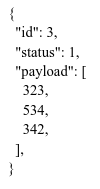
\includegraphics[scale=0.95]{images/create_elements_command_answer_example}}}
\scnaddlevel{1}
\scniselement{ответ на команду создания sc-элементов}
\scntext{интерпретация}{Созданы sc-элементы с хэшами 323, 534 и 342 соответственно. Команда обработана успешно.}
\scnaddlevel{-1}

\scnheader{команда получения соответствующих типов sc-элементов}
\scnidtf{check elements command}
\scnsubset{команда на SC-JSON-коде}
\scnrelfrom{пример}{Пример команды получения соответствующих типов sc-элементов \\ \scneqfile{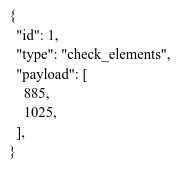
\includegraphics[scale=0.95]{images/check_elements_command_example}}}
\scnaddlevel{1}
\scniselement{команда получения соответствующих типов sc-элементов}
\scnrelfrom{ответ}{Пример ответа на команду получения соответствующих типов sc-элементов}
\scntext{интерпретация}{Получить синтаксические типы sc-элементов с хэшами 885 и 1025.}
\scnaddlevel{-1}
\scnrelfrom{класс команд}{ответ на команду получения соответствующих типов sc-элементов}
\scnnote{Содержимое сообщения \textit{команды получения соответствующих типов sc-элементов} может быть пустым.}

\scnheader{ответ на команду получения соответствующих типов sc-элементов}
\scnidtf{check elements command answer}
\scnsubset{ответ на команду на SC-JSON-коде}
\scnrelfrom{пример}{Пример ответа на команду получения соответствующих типов sc-элементов \\ \scneqfile{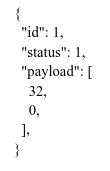
\includegraphics[scale=0.95]{images/check_elements_command_answer_example}}}
\scnaddlevel{1}
\scniselement{ответ на команду получения соответствующих типов sc-элементов}
\scntext{интерпретация}{Типы sc-элементов 32 и 0 соответственно. Команда обработана успешно.}
\scnaddlevel{-1}
\scnnote{Если sc-элемент с указанным хэшем не существует, то его тип будет равен 0.}

\scnheader{команда удаления sc-элементов}
\scnidtf{delete elements command}
\scnsubset{команда на SC-JSON-коде}
\scnrelfrom{пример}{Пример команды удаления sc-элементов \\ \scneqfile{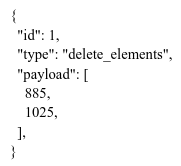
\includegraphics[scale=0.95]{images/delete_elements_command_example}}}
\scnaddlevel{1}
\scniselement{команда удаления sc-элементов}
\scnrelfrom{ответ}{Пример ответа на команду удаления sc-элементов}
\scntext{интерпретация}{Удалить sc-элементы с хэшами 885 и 1025.}
\scnaddlevel{-1}
\scnrelfrom{класс команд}{ответ на команду удаления sc-элементов}
\scnnote{Содержимое сообщения \textit{команды удаления sc-элементов} может быть пустым.}

\scnheader{ответ на команду удаления sc-элементов}
\scnidtf{delete elements command answer}
\scnsubset{ответ на команду на SC-JSON-коде}
\scnrelfrom{пример}{Пример ответа на команду удаления sc-элементов \\ \scneqfile{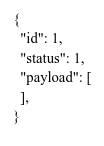
\includegraphics[scale=0.95]{images/delete_elements_command_answer_example}}}
\scnaddlevel{1}
\scniselement{ответ на команду удаления sc-элементов}
\scntext{интерпретация}{Sc-элементы были удалены из sc-памяти успешно.}
\scnaddlevel{-1}
\scnnote{Если sc-элемент с указанным хэшем не существует, ответ на команду будет безуспешным.}

\scnheader{команда обработки ключевых sc-элементов}
\scnidtf{handle keynodes command}
\scnsubset{команда на SC-JSON-коде}
\scnrelfrom{пример}{Пример команды обработки ключевых sc-элементов \\ \scneqfile{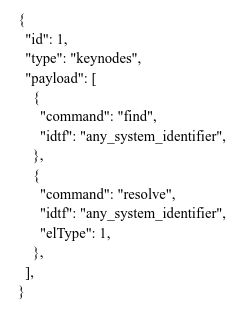
\includegraphics[scale=0.95]{images/handle_keynodes_command_example}}}
\scnaddlevel{1}
\scniselement{команда обработки ключевых sc-элементов}
\scnrelfrom{ответ}{Пример ответа на команду обработки ключевых sc-элементов}
\scntext{интерпретация}{(1) Найти sc-элемент по системному идентификатору "any\_system\_identifier"{}; (2) Разрешить sc-элемент с типом 1 (неуточняемого типа) по системному идентификатору "any\_system\_identifier"{}.}
\scnaddlevel{-1}
\scnrelfrom{класс команд}{ответ на команду обработки ключевых sc-элементов}
\scnnote{Данный класс команд позволяет быстро обращаться к sc-элементам по их системным идентификаторам, поскольку ключевые sc-элементы 	кэшируются на уровне интерфейса.}

\scnheader{ответ на команду обработки ключевых sc-элементов}
\scnidtf{handle keynodes command answer}
\scnsubset{ответ на команду на SC-JSON-коде}
\scnrelfrom{пример}{Пример ответа на команду обработки ключевых sc-элементов \\ \scneqfile{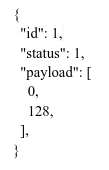
\includegraphics[scale=0.95]{images/handle_keynodes_command_answer_example}}}
\scnaddlevel{1}
\scniselement{ответ на команду обработки ключевых sc-элементов}
\scntext{интерпретация}{Ключевый sc-элемент с системным идентификатором "any\_system\_identifier"{} не был найден, поэтому был создан. хэш нового ключевого sc-элемента - 128. Команда выполнена 	успешно.}
\scnaddlevel{-1}

\scnheader{команда обработки содержимого файлов ostis-системы}
\scnidtf{handle link contents command}
\scnsubset{команда на SC-JSON-коде}
\scnrelfrom{пример}{Пример команды обработки содержимого файлов ostis-системы \\ \scneqfile{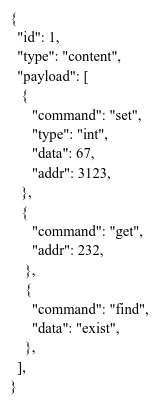
\includegraphics[scale=0.95]{images/handle_link_contents_command_example}}}
\scnaddlevel{1}
\scniselement{команда обработки содержимого файлов ostis-системы}
\scnrelfrom{ответ}{Пример ответа на команду обработки содержимого файлов ostis-системы}
\scntext{интерпретация}{(1) Установить содержимое 67 типа "int"{} в файл ostis-системы с хэшем 3123; (2) Получить содержимое файла ostis-системы с хэшем 232; (3) Найти файлы ostis-системы с содержимым "exist"{}.}
\scnaddlevel{-1}
\scnrelfrom{класс команд}{ответ на команду обработки содержимого файлов ostis-системы}
\scnnote{Стоит отметить, что в случае, если файл ostis-системы уже имеет содержимое, то при установке нового содержимого старое содержимое будет удалено из памяти. Содержимое файла ostis-системы может быть установлено как пустое.}

\scnheader{ответ на команду обработки содержимого файлов ostis-системы}
\scnidtf{handle link contents command answer}
\scnsubset{ответ на команду на SC-JSON-коде}
\scnrelfrom{пример}{Пример ответа на команду обработки содержимого файлов ostis-системы \\ \scneqfile{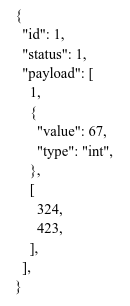
\includegraphics[scale=0.95]{images/handle_link_contents_command_answer_example}}}
\scnaddlevel{1}
\scniselement{ответ на команду обработки содержимого файлов ostis-системы}
\scntext{интерпретация}{(1) Содержимое 67 типа "int"{} было установлено успешно в файл ostis-системы с хэшем 3123; (2) Содержимое файла ostis-системы с хэшем 232 - число 67 целочисленного типа; (3) Файлы ostis-системы с содержимым "exist"{}: 324 и 423.}
\scnaddlevel{-1}

\scnheader{команда поиска sc-конструкций, изоморфных заданному sc-шаблону}
\scnidtf{search template command}
\scnsubset{команда на SC-JSON-коде}
\scnrelfrom{пример}{Пример команды поиска sc-конструкций, изоморфных заданному sc-шаблону \\ \scneqfile{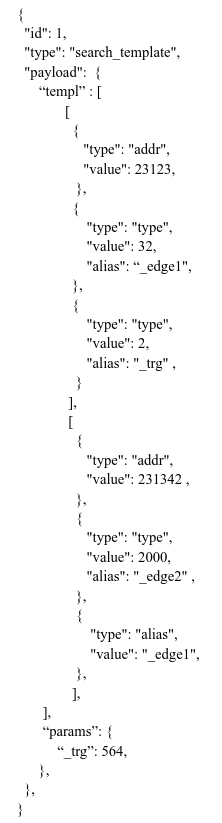
\includegraphics[scale=0.95]{images/search_template_command_example}}}
\scnaddlevel{1}
\scniselement{команда поиска sc-конструкций, изоморфных заданному sc-шаблону}
\scnrelfrom{ответ}{Пример ответа на команду поиска sc-конструкций, изоморфных заданному sc-шаблону}
\scntext{интерпретация}{Найти все такие тройки, в которых первым элементом является sc-элемент c хэшем 23123, третьим sc-элементом является файл ostis-системы неуточняемого константного типа c псевдонимом “\_trg”{}, а вторым элементом - sc-дуга типа sc\_edge\_d\_common c псевдонимом “\_edge1”{}, исходящая от sc-элемента c хэшем 23123 и входящая в файл ostis-системы с псевдонимом “\_trg”{}, и найти все такие тройки, в которых первым элементом является sc-элемент c хэшем 231342, третьим элементов является sc-дуга под псевдонимом “\_edge1”{}, а вторым элементом - sc-дуга типа sc\_edge\_access\_const\_pos\_perm, исходящая от sc-элемента c хэшем 231342 и входящая в sc-дугу “\_edge1”. На место переменной с псевдонимом “\_trg”{} подставить sc-элемент с хэшем 564.}
\scnaddlevel{-1}
\scnrelfrom{класс команд}{ответ на команду поиска sc-конструкций, изоморфных заданному sc-шаблону}
\scnnote{Поиск sс-конструкций по сформированному sc-шаблону осуществляется специализированным модулем, являющимся частью sc-памяти.}

\scnheader{ответ на команду поиска sc-конструкций, изоморфных заданному sc-шаблону}
\scnidtf{search template command answer}
\scnsubset{ответ на команду на SC-JSON-коде}
\scnrelfrom{пример}{Пример ответа на команду поиска sc-конструкций, изоморфных заданному sc-шаблону \\ \scneqfile{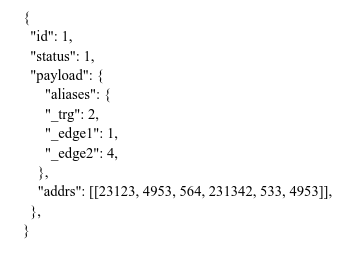
\includegraphics[scale=0.95]{images/search_template_command_answer_example}}}
\scnaddlevel{1}
\scniselement{ответ на команду поиска sc-конструкций, изоморфных заданному sc-шаблону}
\scntext{интерпретация}{Найдена одна sc-конструкция, состоящая из двух троек. хэши sc-элементов в тройках: 23123, 4953, 564 и 231342, 533, 4953 соответственно их расположению в тройках. Команда выполнена успешно.}
\scnaddlevel{-1}
\scnnote{Важно отметить, что sc-шаблон поиска sc-конструкций не может быть пустым.}

\scnheader{команда создания sc-конструкции, изоморфной заданному sc-шаблону}
\scnidtf{generate template command}
\scnsubset{команда на SC-JSON-коде}
\scnrelfrom{пример}{Пример команды создания sc-конструкции, изоморфной заданному sc-шаблону \\ \scneqfile{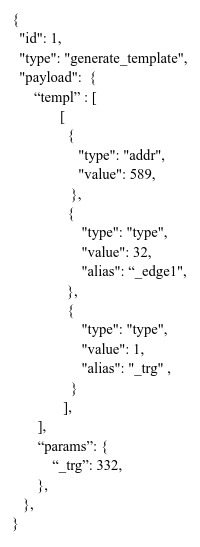
\includegraphics[scale=0.95]{images/generate_template_command_example}}}
\scnaddlevel{1}
\scniselement{команда создания sc-конструкции, изоморфной заданному sc-шаблону}
\scnrelfrom{ответ}{Пример ответа на команду создания sc-конструкции, изоморфной заданному sc-шаблону}
\scntext{интерпретация}{Создать такую тройку, в которой первым элементом является sc-элемент c хэшем 589, третьим sc-элементом является sc-узел неуточняемого типа c псевдонимом “\_trg”{}, а вторым элементом - sc-дуга типа sc\_edge\_d\_common c псевдонимом “\_edge1”{}, исходящая от sc-элемента c хэшем 589 и входящая в sc-узел с псевдонимом “\_trg”{}. На место переменной с псевдонимом “\_trg”{} подставить sc-элемент с хэшем 332.}
\scnaddlevel{-1}
\scnrelfrom{класс команд}{ответ на команду создания sc-конструкции, изоморфной заданному sc-шаблону} 
\scnnote{Создание sс-конструкции по сформированному sc-шаблону осуществляется специализированным модулем, являющимся частью sc-памяти.}

\scnheader{ответ на команду создания sc-конструкции, изоморфной заданному sc-шаблону}
\scnidtf{search template command answer}
\scnsubset{ответ на команду на SC-JSON-коде}
\scnrelfrom{пример}{Пример ответа на команду создания sc-конструкции, изоморфной заданному sc-шаблону \\ \scneqfile{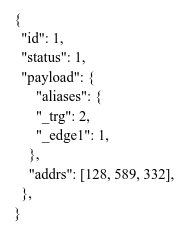
\includegraphics[scale=0.95]{images/generate_template_command_answer_example}}}
\scnaddlevel{1}
\scniselement{ответ на команду создания sc-конструкции, изоморфной заданному sc-шаблону}
\scntext{интерпретация}{Создана одна sc-конструкция, состоящая из одной тройки. хэши sc-элементов в тройке: 128, 589, 332 соответственно их расположению в тройках. Команда выполнена успешно.}
\scnaddlevel{-1}
\scnnote{Важно отметить, что sc-шаблон создания sc-конструкции не может быть пустым.}

\scnheader{команда обработки sc-событий}
\scnidtf{handle events command}
\scnsubset{команда на SC-JSON-коде}
\scnrelfrom{пример}{Пример команды обработки sc-событий \\ \scneqfile{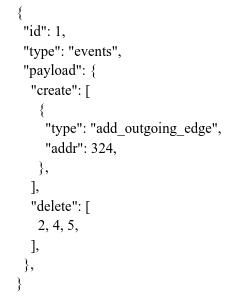
\includegraphics[scale=0.95]{images/handle_events_command_example}}}
\scnaddlevel{1}
\scniselement{команда обработки sc-событий}
\scnrelfrom{ответ}{Пример ответа на команду обработки sc-событий}
\scntext{интерпретация}{(1) Зарегистрировать sc-событие типа "add\_outgoing\_edge"{} по sc-элементу с хэшем 324; (2) Разрегистрировать sc-события с позициями sc-элементов 2, 4 и 5 соответственно.}
\scnaddlevel{-1}
\scnrelfrom{класс команд}{ответ на команду обработки sc-событий}
\scnrelfrom{класс команд}{ответ инициализации sc-события}
\scnnote{\textit{Ответ инициализации sc-события} может производиться несколько раз за разные промежутки времени.}

\scnheader{ответ на команду обработки sc-событий}
\scnidtf{handle events command answer}
\scnsubset{ответ на команду на SC-JSON-коде}
\scnsuperset{SC-JSON-код}
\scnrelfrom{пример}{Пример ответа на команду обработки sc-событий \\ \scneqfile{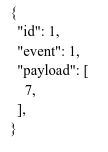
\includegraphics[scale=0.95]{images/handle_events_command_answer_example}}}
\scnaddlevel{1}
\scniselement{ответ на команду обработки sc-событий}
\scntext{интерпретация}{(1) Sc-событие типа "add\_outgoing\_edge"{} по sc-элементу с хэшем 324 было зарегистрировано успешно на 7-ой позиции очереди sc-событий; (2) Sc-события под позициями 2, 4, 5 удалены успешно.}
\scnaddlevel{-1}

\scnheader{ответ инициализации sc-события}
\scnidtf{init event command answer}
\scnsubset{ответ на команду на SC-JSON-коде}
\scnrelfrom{пример}{Пример ответа инициализации sc-события \\ \scneqfile{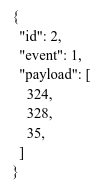
\includegraphics[scale=0.95]{images/init_event_command_answer_example}}}
\scnaddlevel{1}
\scniselement{ответ инициализации sc-события}
\scntext{интерпретация}{Sc-событие было инициализировано успешно: добавлена выходящая sc-дуга с хэшем 328 из зарегистрированного sc-элемента с хэшем 324 в sc-элемент c хэшем 35. Статус sc-события - 1.}
\scnaddlevel{-1}

\scnendstruct \scninlinesourcecommentpar{Завершили представление \textit{Синтаксиса SC-JSON-кода}}

\scnheader{Серверная система на основе Websocket, обеспечивающая доступ к sc-памяти платформы интерпретации sc-моделей при помощи команд SC-JSON-кода}
\scnidtf{Система, работающая по принципам Websocket и предоставляющая параллельно-асинхронный многоклиентский доступ к sc-памяти платформы интерпретации sc-моделей при помощи SC-JSON-кода}
\scnidtf{SC-JSON-сервер}
\scntext{часто используемый неосновной внешний идентификатор sc-элемента}{SC-сервер}
\scniselement{многократно используемый компонент ostis-систем}
\scniselement{атомарный многократно используемый компонент ostis-систем}
\scniselement{зависимый многократно используемый компонент ostis-систем}
\scnrelto{компонент системы}{Программный вариант реализации платформы интерпретации sc-моделей компьютерных систем}
\scnrelfromlist{авторы}{Зотов Н. В.}
\scnrelfromlist{используемый язык программирования}{C;C++}
\scnrelfromlist{используемый язык}{SC-JSON-код}
\scnrelfromset{зависимости компонента}{
Библиотека программных компонентов для обработки и, задающее синтаксис json-текстов JSON for Modern C++ версии 3.10.5\\
\scnaddlevel{1}
	\scnidtf{nlohmann-json 3.10.5}
	\scnrelto{версия компонента}{Библиотека программных компонентов для обработки и, задающее синтаксис json-текстов JSON for Modern C++}
	\scnaddlevel{1}
		\scnidtf{nlohmann-json}
		\scniselement{многократно используемый компонент ostis-систем}
		\scniselement{неатомарный многократно используемый компонент ostis-систем}
		\scniselement{зависимый многократно используемый компонент ostis-систем}
		\scntext{адрес хранилища}{https://github.com/nlohmann/json}
		\scnaddlevel{1}
			\scniselement{адрес хранилища на GitHub}
		\scnaddlevel{-1}
		\scntext{скрипт установки}{
			sudo add-apt-repository universe\\
			sudo apt-get update\\
			sudo apt-get install -y nlohmann-json3-dev
		}
		\scnaddlevel{1}
			\scniselement{скрипт на языке Bash}
			\scniselement{скрипт на языке Bash, поддерживаемый семейством операционных систем UNIX}
		\scnaddlevel{-1}
		\scntext{скрипт установки}{
			brew install nlohmann-json
		}
		\scnaddlevel{1}
			\scniselement{скрипт на языке Bash}
			\scniselement{скрипт на языке Bash, поддерживаемый семейством операционных систем MaсOS}
		\scnaddlevel{-1}
	\scnaddlevel{-1}
\scnaddlevel{-1}; 
Библиотека кросс-платформенных программных компонентов для реализации серверных приложений на основе Websocket WebSocket++ версии 0.8.2\\
\scnaddlevel{1}
	\scnidtf{websocketcpp 0.8.2}
	\scnrelto{версия компонента}{Библиотека кросс-платформенных программных компонентов для реализации серверных приложений на основе Websocket WebSocket++}
	\scnaddlevel{1}
		\scnidtf{websocketcpp}
		\scniselement{многократно используемый компонент ostis-систем}
		\scniselement{неатомарный многократно используемый компонент ostis-систем}
		\scniselement{зависимый многократно используемый компонент ostis-систем}
		\scntext{адрес хранилища}{https://github.com/zaphoyd/websocketpp}
		\scnaddlevel{1}
			\scniselement{адрес хранилища на GitHub}
		\scnaddlevel{-1}
		\scntext{скрипт установки}{
			sudo apt-get update\\
			sudo apt-get install -y libwebsocketpp-dev
		}
		\scnaddlevel{1}
			\scniselement{скрипт на языке Bash}
			\scniselement{скрипт на языке Bash, поддерживаемый семейством операционных систем UNIX}
		\scnaddlevel{-1}
		\scntext{скрипт установки}{
			brew install libwebsocketpp
		}
		\scnaddlevel{1}
			\scniselement{скрипт на языке Bash}
			\scniselement{скрипт на языке Bash, поддерживаемый семейством операционных систем MaсOS}
		\scnaddlevel{-1}
	\scnaddlevel{-1}
\scnaddlevel{-1};
Программный компонент настройки программных компонентов ostis-систем версии 0.1.0\\
\scnaddlevel{1}
	\scnidtf{sc-config-utils 0.1.0}
	\scnrelto{версия компонента}{Программный компонент настройки программных компонентов ostis-систем}
	\scnaddlevel{1}
		\scnidtf{sc-config-utils}
		\scniselement{многократно используемый компонент ostis-систем}
		\scniselement{неатомарный многократно используемый компонент ostis-систем}
		\scniselement{зависимый многократно используемый компонент ostis-систем}
		\scnrelfromlist{авторы}{Зотов Н. В.\\; Насевич П. Е.\\; Хорошавин В. Д.}
		\scntext{адрес хранилища}{https://github.com/ostis-ai/sc-machine/tree/main/sc-tools/sc-config-utils}
		\scnaddlevel{1}
			\scniselement{адрес хранилища на GitHub}
		\scnaddlevel{-1}
	\scnaddlevel{-1}
\scnaddlevel{-1};
Программная модель sc-памяти версии 0.6.1
\scnidtf{sc-machine 0.6.1}
\scnaddlevel{1}
	\scnrelto{версия компонента}{Программная модель sc-памяти}
\scnaddlevel{-1}
}
\scntext{адрес хранилища}{https://github.com/ostis-ai/sc-machine/tree/main/sc-tools/sc-server}
\scnaddlevel{1}
	\scniselement{адрес хранилища на GitHub}
\scnaddlevel{-1}
\scnexplanation{\textit{Серверная система на основе Websocket, обеспечивающая доступ к sc-памяти платформы интерпретации sc-моделей при помощи команд SC-JSON-кода}, представляет собой интерпретатор команд и ответов на них \textit{SC-JSON-кода} на программное представление sc-конструкций в sc-памяти при помощи Библиотеки программных компонентов для обработки и, задающее синтаксис json-текстов JSON for Modern C++ и Библиотека кросс-платформенных программных компонентов для реализации серверных приложений на основе Websocket WebSocket++, а также обеспечивается комплексным тестовым покрытием посредством программных фреймворков Google Tests и Google Benchmark Tests. Библиотека программных компонентов для обработки и, задающее синтаксис json-текстов JSON for Modern C++ имеет богатый, удобный и быстродействующий функционал, необходимый для реализации подобных компонентов ostis-систем, а Библиотеки кросс-платформенных программных компонентов для реализации серверных приложений на основе Websocket WebSocket++ позволяет элегантно проектировать серверные системы без использовании избыточных зависимостей и решение. Настройка программного компонента осуществляется с помощью \textit{Программного компонента настройки программных компонентов ostis-систем} и скриптов языков CMake и Bash.}
\scnexplanation{Стоит отметить, что текущая реализация \textit{Серверной системы на основе Websocket, обеспечивающая доступ к sc-памяти платформы интерпретации sc-моделей при помощи команд SC-JSON-кода} не является первой в своём роде и заменяет предыдущую её реализацию, написанную на языке Python. Причиной такой замены состоит в следующем:
	\begin{scnitemize}
		\item предыдущая реализация \textit{Серверной системы на основе Websocket, обеспечивающая доступ к sc-памяти платформы интерпретации sc-моделей при помощи команд SC-JSON-кода}, реализованная на языке программирования Python, зависит от библиотеки Boost Python, предоставляемой сообществом по развитию и коллаборации языков С++ и Python. Дело в том, что такое решение требует поддержки механизма интерпретации программного кода на языке Python на язык С++, что является избыточным и необоснованным, поскольку большая часть программного кода \textit{\textbf{Программного варианта реализации платформы интерпретации sc-моделей компьютерных систем}} реализована на языках С и С++. Новая реализация описываемой программной системы позволяет избавиться от использования ёмких и ресурсозатратных библиотек (например, boost-python-lib, llvm) и языка Python;
		\item при реализации распределённых подсистем важную роль играет скорость обработки знаний, то есть возможность быстро и срочно отвечать на запросы пользователя. Качество доступа к sc-памяти посредством реализованной \textit{Подсистемы взаимодействия с sc-памятью на основе языка JSON} должно быть соизмеримо с качеством доступа к sc-памяти при помощи специализированного программного интерфейса API, реализованного на том же языке программирования, что и сама система. Новая реализация позволяет повысить скорость обработки запросов \textit{Подсистемой взаимодействия с sc-памятью на основе языка JSON}, в том числе и обработка знаний, не менее чем в 1,5 раза по сравнению с предыдущим вариантом реализации этой подсистемы.
	\end{scnitemize}
}
\scnrelfrom{формальная модель}{Модель \textit{Серверной системы на основе Websocket, обеспечивающая доступ к sc-памяти платформы интерпретации sc-моделей при помощи команд SC-JSON-кода}}
\scnrelfromlist{характеристика}{
	\scnfileitem{\textit{Серверная система на основе Websocket, обеспечивающая доступ к sc-памяти платформы интерпретации sc-моделей при помощи команд SC-JSON-кода} обеспечивает многофункциональный доступ к sc-памяти ostis-системы и удовлетворяет требованиям своей модели. С точки зрения прагматики, программный компонент имеет такой же специализированный программный интерфейс, как и \textit{Программная модель sc-памяти}, однако взаимодействие с ним осуществляется посредством сети.}\\;
	\scnfileitem{Реализованный программный компонент позволяет многопользовательский асинхронный доступ к sc-памяти. В ходе тестирования sc-сервера выяснилось, что его реализация позволяет обрабатывать запросы 1000 клиентских систем. В связи с необходимостью обеспечения параллельного доступа к sc-памяти на уровне реализации программного компонента были добавлены блоки синхронизации. Среди таких можно заметить очередь команд на обработку системой - вне зависимости от того сколько клиентских систем и в каком количестве они отправляют команды на обработку, все команды добавляются в очередь - такое решение позволит обойти проблемы взаимодействия блоков синхронизации на уровне sc-памяти. При этом серверную систему невозможно отключить до тех пор, пока очередь команд имеет какие-нибудь элементы. Также серверная система продолжает работать, если в списке идентификаторов клиентских систем остались некоторые идентификаторы этих клиентских систем. Эти функции обуславливаются необходимостью поддержки атомарности запросов, обрабатываемых системой.}\\;
	\scnfileitem{В процессе тестирования реализации \textit{Серверной системы на основе Websocket, обеспечивающая доступ к sc-памяти платформы интерпретации sc-моделей при помощи команд SC-JSON-кода}, были получены оценки скорости обработки запросов этим компонентом. При нагрузочном тестировании использовалась тестовая клиентская система, написанная на С++ и не имеющая функционала обработки текстов SC-JSON-кода. В результате тестирования было выяснено, что при отправке серверной системы 1000 различных команд: команд создания sc-элементов, команд обработки содержимого файлов ostis-системы и команд удаления sc-элементов, время потраченное на их обработку не превышало 0,2 секунды. При этом в отдельных случаях на обработку 1000 команд создания sc-элементов уходило не более 0,14 секунды, команд удаления sc-элементов - не более 0,07 секунды, команд обработки содержимого файлов ostis-системы - не более 0,27 секунды, команд поиска sc-конструкций, изоморфных заданному sc-шаблону - не более 0,45 секунды.}
}

\scnheader{Модель \textit{Серверной системы на основе Websocket, обеспечивающая доступ к sc-памяти платформы интерпретации sc-моделей при помощи команд SC-JSON-кода}}
\scnreltovector{декартово произведение}{
	\scnnonamednode\\
	\scnaddlevel{1}
		\scnreltovector{декартово произведение}{
			\scnnonamednode\\
			\scnaddlevel{1}
				\scnreltovector{декартово произведение}{
					\scnnonamednode\\
					\scnaddlevel{1}
					\scnreltovector{декартово произведение}{
						функция создания sc-элементов по их описаниям: типам и инцидентным sc-элементам*\\;
						функция получения соответствующих синтаксических типов sc-элементов*
					}
					\scnaddlevel{-1}\\;
					\scnnonamednode\\
					\scnaddlevel{1}
					\scnreltovector{декартово произведение}{
						функция проверки существования sc-элементов в sc-памяти*\\;
						функция получения ключевого sc-элемента по системному идентификатору*
					}
					\scnaddlevel{-1}
				}
			\scnaddlevel{-1}\\;
			\scnnonamednode\\
			\scnaddlevel{1}
				\scnreltovector{декартово произведение}{
					\scnnonamednode\\
					\scnaddlevel{1}
					\scnreltovector{декартово произведение}{
						функция разрешения ключевого sc-элемента по системному идентификатору*\\;
						функция установки содержимого в файл ostis-системы*
					}
					\scnaddlevel{-1}\\;
					\scnnonamednode\\
					\scnaddlevel{1}
					\scnreltovector{декартово произведение}{
						функция получения содержимого из файлов ostis-системы*\\;
						функция получения файлов ostis-системы по содержимому*
					}
					\scnaddlevel{-1}
				}
			\scnaddlevel{-1}
		}
	\scnaddlevel{-1}\\;
	\scnnonamednode\\
	\scnaddlevel{1}
		\scnreltovector{декартово произведение}{
			\scnnonamednode\\
			\scnaddlevel{1}
				\scnreltovector{декартово произведение}{
					функция поиска sc-конструкций, изоморфных заданному sc-шаблону, состоящего из троек, специфицированных инцидентными sc-элементами и/или синтаксическими типами и/или идентификаторами и/или псевдонимами их sc-элементов*\\;
					функция создания sc-конструкции, изоморфной заданному sc-шаблону, состоящего из троек, специфицированных инцидентными sc-элементами и/или синтаксическими типами и/или идентификаторами и/или псевдонимами их sc-элементов*
				}
				\scnaddlevel{-1}\\;
				\scnnonamednode\\
				\scnaddlevel{1}
				\scnreltovector{декартово произведение}{
					функция подписки sc-события на sc-элемент*\\;
					функция отмены подписки sc-события на sc-элемент*
				}
			\scnaddlevel{-1}
		}
	\scnaddlevel{-1}
}
\scnexplanation{\textit{Модель Серверной системы на основе Websocket, обеспечивающая доступ к sc-памяти платформы интерпретации sc-моделей при помощи команд SC-JSON-кода} описывает необходимы и достаточный программный интерфейс для взаимодействия c sc-памятью. В общем случае описывает функциональные возможности не только \textit{Серверной системы на основе Websocket, обеспечивающая доступ к sc-памяти платформы интерпретации sc-моделей при помощи команд SC-JSON-кода}, но клиентских систем взаимодействующих с ней, поскольку зачастую эти клиентские системы включают специализированный программный интерфейс, схожий с интерфейсом серверной системы, но на другом языке программирования.}
\scneqtoset{
	функция создания sc-элементов по их описаниям: типам и инцидентным sc-элементам*\\
	\scnaddlevel{1}
		\scnreltovector{декартово произведение}{
			\scnnonamednode\\
			\scnaddlevel{1}
			\scnreltovector{декартово произведение}{
				Множество всех синтаксических типов sc-элементов\\;
				Множество всех sc-элементов, имеющих инцидентные sc-элементы в sc-памяти
			}
			\scnaddlevel{-1}\\;
			Множество всех sc-элементов, хранящихся в sc-памяти
		}
		\scnnote{Создается sc-элемент заданного синтаксического типа из Множества всех синтаксических типов sc-элементов и имеющий заданные связи с заданными элементами из Множества всех sc-элементов, имеющих инцидентные sc-элементы в sc-памяти, дополняя Множество всех sc-элементов, хранящихся в sc-памяти.}
	\scnaddlevel{-1};
	функция получения соответствующих синтаксических типов sc-элементов*\\
	\scnaddlevel{1}
		\scnreltovector{декартово произведение}{
			Множество всех sc-элементов, хранящихся в sc-памяти\\;
			Множество всех синтаксических типов sc-элементов
		}
		\scnnote{У каждого sc-элемента из Множества всех sc-элементов, хранящихся в sc-памяти, можно получить соответствующий синтаксический тип из Множества всех синтаксических типов sc-элементов.}
	\scnaddlevel{-1};
	функция проверки существования sc-элементов в sc-памяти*\\
	\scnaddlevel{1}
		\scnreltovector{декартово произведение}{
			Множество всех sc-элементов, хранящихся в sc-памяти\\;
			Множество, состоящее из знаков истины и лжи
		}
		\scnnote{Каждый sc-элемент из Множества всех sc-элементов, хранящихся в sc-памяти, должен находиться в sc-памяти.}
	\scnaddlevel{-1};
	функция получения ключевого sc-элемента по системному идентификатору*\\
	\scnaddlevel{1}
		\scnreltovector{разность множеств}{
			\scnnonamednode\\
			\scnaddlevel{1}
				\scnreltoset{объединение}{
					\scnnonamednode\\
					\scnaddlevel{1}
					\scnreltovector{декартово произведение}{
						Множество всех sc-элементов, хранящихся в sc-памяти\\;
						Множество всех ключевых sc-элементов, хранящихся в sc-памяти
					}
					\scnaddlevel{-1}\\;
					\scnnonamednode\\
					\scnaddlevel{1}
					\scnreltovector{декартово произведение}{
						Множество всех системных идентификаторов sc-элементов, хранящихся в файловом хранилище\\;
						Множество всех ключевых sc-элементов, хранящихся в sc-памяти
					}
					\scnaddlevel{-1}
				}
			\scnaddlevel{-1}\\;
			функция разрешения ключевого sc-элемента по системному идентификатору*
		}
		\scnnote{Каждый ключевой sc-элемент из Множества всех ключевых sc-элементов, хранящихся в sc-памяти, является sc-элементом Множества всех sc-элементов, хранящихся в sc-памяти, и имеет, по крайней мере, системный идентификатор из Множества всех системных идентификаторов sc-элементов, хранящихся в файловом хранилищеs.}
	\scnaddlevel{-1};
	функция разрешения ключевого sc-элемента по системному идентификатору*\\
	\scnaddlevel{1}
		\scnreltovector{разность множеств}{
			\scnnonamednode\\
			\scnaddlevel{1}
			\scnreltoset{объединение}{
				\scnnonamednode\\
				\scnaddlevel{1}
				\scnreltovector{декартово произведение}{
					Множество всех sc-элементов, хранящихся в sc-памяти\\;
					Множество всех ключевых sc-элементов, хранящихся в sc-памяти
				}
				\scnaddlevel{-1}\\;
				\scnnonamednode\\
				\scnaddlevel{1}
				\scnreltovector{декартово произведение}{
					Множество всех системных идентификаторов sc-элементов, хранящихся в файловом хранилище\\;
					Множество всех ключевых sc-элементов, хранящихся в sc-памяти
				}
				\scnaddlevel{-1}
			}
			\scnaddlevel{-1}\\;
			функция получения ключевого sc-элемента по системному идентификатору*
		}
		\scnnote{Из каждого sc-элемента Множества всех sc-элементов, хранящихся в sc-памяти, можно получить ключевой sc-элемент Множества всех ключевых sc-элементов, хранящихся в sc-памяти, зная, по крайней мере, его системный идентификатор из Множества всех системных идентификаторов sc-элементов, хранящихся в файловом хранилище.}
	\scnaddlevel{-1};
	функция установки содержимого в файл ostis-системы*\\
	\scnaddlevel{1}
		\scnreltovector{декартово произведение}{
			\scnnonamednode\\
			\scnaddlevel{1}
			\scnreltovector{декартово произведение}{
				Множество всех файлов ostis-системы, хранящихся в sc-памяти\\;
				Множество внешних знаков, являющихся содержимым файлов ostis-системы, хранящиеся в файловом хранилище
			}
			\scnaddlevel{-1}\\;
			Множество, состоящее из знаков истины и лжи
		}
		\scnnote{В каждый sc-элемент из Множества всех файлов ostis-системы, хранящихся в sc-памяти\\ может быть установлено содержимое из Множества всего содержимого файлов ostis-системы, хранящегося в файловом хранилище.}
	\scnaddlevel{-1};
	функция получения содержимого из файлов ostis-системы*\\
	\scnaddlevel{1}
		\scnreltovector{декартово произведение}{
			Множество всех файлов ostis-системы, хранящихся в sc-памяти\\;
			Множество внешних знаков, являющихся содержимым файлов ostis-системы, хранящиеся в файловом хранилище
		}
		\scnnote{Из каждого файла ostis-системы Множества всех файлов ostis-системы, хранящихся в sc-памяти, можно получить содержимое, принадлежащее Множеству внешних знаков, являющихся содержимым файлов ostis-системы, хранящиеся в файловом хранилище.}
	\scnaddlevel{-1};
	функция получения файлов ostis-системы по содержимому*\\
	\scnaddlevel{1}
		\scnreltovector{декартово произведение}{
			Множество внешних знаков, являющихся содержимым файлов ostis-системы, хранящиеся в файловом хранилище\\;
			Множество всех файлов ostis-системы, хранящихся в sc-памяти
		}
		\scnnote{По содержимому из Множества внешних знаков, являющихся содержимым файлов ostis-системы, хранящиеся в файловом хранилище, можно получить подмножество файлов ostis-системы из Множества всех файлов ostis-системы, хранящихся в sc-памяти, в которые установлено это содержимое.}
	\scnaddlevel{-1};
	функция поиска sc-конструкций, изоморфных заданному sc-шаблону, состоящего из троек, специфицированных инцидентными sc-элементами и/или синтаксическими типами и/или идентификаторами и/или псевдонимами их sc-элементов*\\
	\scnaddlevel{1}
		\scnreltovector{разность множеств}{
			\scnnonamednode\\
			\scnaddlevel{1}
				\scnreltovector{декартово произведение}{
					\scnnonamednode\\
					\scnaddlevel{1}
					\scnreltovector{декартово произведение}{
						\scnnonamednode\\
						\scnaddlevel{1}
						\scnreltovector{декартово произведение}{
							Множество всех sc-элементов, хранящихся в sc-памяти\\;
							Множество всех синтаксических типов sc-элементов
						}
						\scnaddlevel{-1}\\;
						\scnnonamednode\\
						\scnaddlevel{1}
						\scnreltovector{декартово произведение}{
							Множество всех sc-элементов, имеющих инцидентные sc-элементы в sc-памяти\\;
							Множество всех идентификаторов sc-элементов, хранящихся в файловом хранилище
						}
						\scnaddlevel{-1}
					}
					\scnaddlevel{-1}\\;
					Множество всех sc-структур
				}
			\scnaddlevel{-1}\\;
			функция создания sc-конструкции, изоморфной заданному sc-шаблону, состоящего из троек, специфицированных инцидентными sc-элементами и/или синтаксическими типами и/или идентификаторами и/или псевдонимами их sc-элементов*
		}
		\scnnote{По синтаксическим типам sc-элементов из Множества всех синтаксических типов sc-элементов и/или самим sc-элементам из Множества всех sc-элементов, хранящихся в sc-памяти, связанными с sc-элементами, у которых известны синтаксические типы из Множества всех синтаксических типов sc-элементов, в том числе инцидентным sc-элементами из Множества всех sc-элементов, имеющих инцидентные sc-элементы в sc-памяти, и/или идентификаторам (в том числе псевдонимам) sc-элементов Множества всех идентификаторов sc-элементов, хранящихся в файловом хранилище можно найти sc-структуры, принадлежащие Множеству всех sc-структур и состоящие из всех этих sc-элементов.}
	\scnaddlevel{-1};
	функция создания sc-конструкции, изоморфной заданному sc-шаблону, состоящего из троек, специфицированных инцидентными sc-элементами и/или синтаксическими типами и/или идентификаторами и/или псевдонимами их sc-элементов*\\
	\scnaddlevel{1}
		\scnreltovector{разность множеств}{
			\scnnonamednode\\
			\scnaddlevel{1}
				\scnreltovector{декартово произведение}{
					\scnnonamednode\\
					\scnaddlevel{1}
					\scnreltovector{декартово произведение}{
						\scnnonamednode\\
						\scnaddlevel{1}
						\scnreltovector{декартово произведение}{
							Множество всех sc-элементов, хранящихся в sc-памяти\\;
							Множество всех синтаксических типов sc-элементов
						}
						\scnaddlevel{-1}\\;
						\scnnonamednode\\
						\scnaddlevel{1}
						\scnreltovector{декартово произведение}{
							Множество всех sc-элементов, имеющих инцидентные sc-элементы в sc-памяти\\;
							Множество всех идентификаторов sc-элементов, хранящихся в файловом хранилище
						}
						\scnaddlevel{-1}
					}
					\scnaddlevel{-1}\\;
					Множество всех sc-структур
				}
			\scnaddlevel{-1}\\;
			функция поиска sc-конструкций, изоморфных заданному sc-шаблону, состоящего из троек, специфицированных инцидентными sc-элементами и/или синтаксическими типами и/или идентификаторами и/или псевдонимами их sc-элементов*
		}
		\scnnote{По синтаксическим типам sc-элементов из Множества всех синтаксических типов sc-элементов и/или самим sc-элементам из Множества всех sc-элементов, хранящихся в sc-памяти, связанными с sc-элементами, у которых известны синтаксические типы из Множества всех синтаксических типов sc-элементов, в том числе инцидентным sc-элементами из Множества всех sc-элементов, имеющих инцидентные sc-элементы в sc-памяти, и/или идентификаторам (в том числе псевдонимам) sc-элементов Множества всех идентификаторов sc-элементов, хранящихся в файловом хранилище всегда можно создать sc-структуру, дополняющую Множество всех sc-структур и состоящую из всех этих sc-элементов.}
	\scnaddlevel{-1};
	функция подписки sc-события на sc-элемент\\
	\scnaddlevel{1}
		\scnreltovector{декартово произведение}{
			\scnnonamednode\\
			\scnaddlevel{1}
			\scnreltovector{декартово произведение}{
				Множество всех sc-элементов, храняшихся в sc-памяти\\;
				Множество всех возможных типов sc-событий в sc-памяти
			}
			\scnaddlevel{-1}\\;
			Множество всех sc-событий, зарегистрированных в sc-памяти
		}
		\scnnote{На каждый sc-элемент Множества всех sc-элементов, храняшихся в sc-памяти можно подписать sc-cобытие из Множества всех sc-событий, зарегистрированных в sc-памяти типа из Множества всех sc-событий, зарегистрированных в sc-памяти.}
	\scnaddlevel{-1};
	функция отмены подписки sc-события на sc-элемент\\
	\scnaddlevel{1}
		\scnreltovector{декартово произведение}{
			\scnnonamednode\\
			\scnaddlevel{1}
			\scnreltovector{декартово произведение}{
				Множество всех sc-событий, зарегистрированных в sc-памяти\\;
				Множество всех sc-элементов, храняшихся в sc-памяти
			}
			\scnaddlevel{-1}\\;
			Множество, состоящее из знаков истины и лжи
		}
		\scnnote{На каждый sc-элемент Множества всех sc-элементов, храняшихся в sc-памяти можно отписать от sc-cобытия из Множества всех sc-событий, зарегистрированных в sc-памяти.}
	\scnaddlevel{-1}
}

\bigskip
\scnendstruct \scninlinesourcecommentpar{Завершили описание \textit{Подсистемы взаимодействия c sc-памятью на основе языка JSON}}